\section{Internal Combustion Engine Simulator}
%
ICESym es un simulador de motores de combustión interna que  utiliza modelos 0D
para la cámara de combustión y 1D para el flujo a través del sistema de
intercambio de gases.
%
Esta combinación permite evaluar la \emph{performance} de un motor a un costo
computacional relativamente bajo; además la implementación de entrada y salida
de datos facilita utilizar el simulador como una \emph{caja negra}.
%
Esta característica permite incluir al simulador en un \emph{script} como una
función, a la cual se le otorga un conjunto de parámetros de entrada y devuelve
los resultados de la simulación en un formato que permite la lectura y
evaluación de los mismos.

ICESym contiene en su código las rutinas necesarias para simular el ciclo
operativo y la geometría del MRCVC.
%
Se realizaron modificaciones menores para facilitar la ejecución en conjunto con
el optimizador, algunas de estas modificaciones fueron:
%
\begin{enumerate}
    \item Modificar el formato de los archivos de salida, con el fin de reducir
el tamaño de los archivos de salida, facilitar la lectura y el procesamiento de
datos.
    \item Incluir una opción para elegir entre un modelo de $C_D$ de una o dos
variables.
    \item Modificar el área de referencia, ver Ecuación~\ref{eq:fv}.
    \item Agregar un esquema de interpolación bilineal que permita trabajar con
el modelo de $C_{D}$ de dos variables.
\end{enumerate}


\section{Modificaciones a ICESym}
%%%%%%%%%%%%%%%%%%%%%%%%%%%%%%%%%%%%%%%%%%%%%%%%%%%%%%%%%%%%%%%%%%%%%%%%%%%%%%%
\subsection{Flujo a Través de los Puertos}
%
Se introdujo una opción para poder ejecutar ICESym con un modelo del coeficiente
de descarga que dependa de dos variables: diferencia de presión y \emph{alzada}
o apertura del puerto, $C_D = f(lv; \Delta P)$.
%
Esto significó agregar un \emph{switch} en el código que permita seleccionar
entre un modelo de una o dos variables, con el agregado de las instrucciones de
lectura de datos y armado de un arreglo bidimensional que contiene los valores
del mapa de $C_{D}$ en un orden dado.
%
Con esto se construye un mapa del coeficiente de descarga de la forma $C_D =
f(lv, \Delta P)$, que se utiliza para calcular el área efectiva del puerto.

\nomenclature[F]{\(\Delta P\)}{Diferencia de presión a través de un puerto}

Independientemente de la cantidad de variables que formen parte del coeficiente
de descarga, a ICESym se introduce un vector para el caso 1D y matriz para el
caso 2D.
%
El esquema de interpolación bilineal implementado requiere de una malla
rectangular.
%
Se reutilizó el código existente para el caso 1D y se realiza una interpolación
lineal entre dos valores en planos con datos conocidos, como se ve en la
Figura~\ref{fig:interp_bilineal}.

\begin{figure}
    \centering
    \includegraphics[width=0.7\textwidth]{interpolacion_bilineal.png}
    %
    \caption{Interpolación bilineal\protect\footnotemark}\label{fig:interp_bilineal}
    % \footnote{A}}
\end{figure}

\footnotetext{\url{https://stackoverflow.com/questions/8808996/bilinear-interpolation-to-enlarge-bitmap-images}}

Si bien hay otros métodos de interpolación para estimar el valor de $C_D$ a
partir de una nube de puntos, este método es sencillo y da resultados
satisfactorios.
%
En la Figura~\ref{fig:bilineal} se muestra a modo de ejemplo el error obtenido
con este método para interpolar una función de prueba
$f=\sin\left(\sqrt{x^2 + y^2}\right)$.

\begin{figure}
    \centering
    \includegraphics[width=0.7\textwidth]{bilineal.png}
    \caption{Interpolación bilineal de $\sin(\sqrt{x^2 + y^2})$}\label{fig:bilineal}
\end{figure}

La malla rectangular requerida para la interpolación bilineal del mapa de
$C_{D}$ se realizó a partir de los valores resultantes de las flujometrías con
\emph{OpenFOAM}~\parencite{openfoam}.
%
Debido al costo computacional que requieren las flujometrías, solo una cantidad
reducida de puntos se obtendrá con este método.
%
Se tiene como punto de partida una malla no rectangular, por lo que se utiliza
un método intermedio para obtener una matriz de puntos que pueda ser leída por
la interpolación bilineal.

Se probaron dos métodos para realizar esta interpolación, el método del punto más
cercano (MC) y la interpolación por la suma de la inversa de la distancia o IDW por
sus siglas en inglés (\emph{Inverse Distance Weighting}).
%
Estos se combinan con métodos de suavizado de promedio móvil con los $S$ valores
más cercanos.
%
Con este método cada valor original de la matriz se reemplaza por el promedio
aritmético de los valores a una distancia $S$ de cada celda evaluada.
%
En la Figura~\ref{fig:suavizado_promedio} se muestra este proceso para una
matriz de $5\times5$.

\begin{figure}
    \centering
    \includegraphics[]{/mapa_cd/suavizado.pdf}
    \caption{Suavizado por promedio con celdas vecinas, S=1}\label{fig:suavizado_promedio}
\end{figure}


El método del punto más cercano consiste en asignar para cada par $(x, y)$ el
valor conocido más cercano, ver Algoritmo~\ref{algo:mas_cercano}.

\begin{algorithm}
 \caption{Interpolación por punto más cercano}\label{algo:mas_cercano}
    \KwIn{\\
        $V_x, V_y$: valores de $x, y$ en los que se conoce el valor en $z$.\\
        $V_z$: valores conocidos de $z$.\\
        $I_x$: $n$ puntos de $x$ donde se quiere interpolar\\
        $I_y$: $m$ puntos de $y$ donde se quiere interpolar\\
        }

    \KwResult{Devuelve una matriz $I_{[n,m]}$ con los valores interpolados,
      donde a cada punto $I(x,y)$ se le asigna al valor de $v_z$ más cercano
      conocido. Da como resultado superficies escalonadas.}

    \BlankLine
     $I=zeros_{[n,m]}$\;
     \For{$i \gets 0$\KwTo$n$}{
        \For{$j \gets 0$\KwTo$m$}{
          $d = \sqrt{{(V_x - I_{xi})}^2 + {(V_y - I_{yj})}^2}$\;
            $I[i,j] = v_z[\min(d)]$\;
        }
     }
\end{algorithm}

La interpolación por IDW consiste en asignar a cada punto el resultado de un
promedio de los valores cercanos, ponderado por la distancia elevado a un
exponente arbitrario $p$.
%
Cuanto más grande el valor de $p$, más sensible es el método a los valores
cercanos.
%
La ecuación del promedio es la~(\ref{eq:idw}) y en el Algoritmo~\ref{algo:IDW}
se presenta el esquema utilizado.
%

\begin{equation} \label{eq:idw}
    f_p = \frac{\sum_{i=1}^{n} \frac{z_i}{d_i^p}} {\sum_{i=1}^{n}
    \frac{1}{d_i^p}}
\end{equation}

En la Figura~\ref{fig:mapas_interpolados} se muestra una comparación de ambos
métodos, para una malla de $C_{D}=f(\Delta P, l_{v})$ generada al azar.

\begin{algorithm}
    \caption{Interpolación IDW}\label{algo:IDW}
    \KwIn{\\
        $V_x, V_y$: valores de $x, y$ en los que se conoce el valor en $z$.\\
        $V_z$: valores conocidos de $z$.\\
        $I_x$: $n$ puntos de $x$ donde se quiere interpolar\\
        $I_y$: $m$ puntos de $y$ donde se quiere interpolar\\
        $p$: potencia a la que se eleva cada peso\\
        }

    \KwResult{Interpolación ponderada por inverso de la distancia. Dependiendo
      del valor de $p$, se obtienen valores más o menos suavizados.}

    \BlankLine
    $I=zeros_{[n,m]}$\;
    \For{$i \gets 0$\KwTo$n$}{
        \For{$j$\gets 0 \KwTo$m$}{
          $d = {\left[{(V_x - I_{xi})}^2 +{(V_y - I_{yj})}^2\right]}^{\frac{p}{2}}$\;
          \eIf{$\exists i : d[i] = 0$}{
            $I[i, j] = V_z[i]$\;
          }{
            $I[i,j] = \frac{\sum{V_{zi}/d_i}}{\sum \frac{1}{d}}$\;
          }
        }
     }
\end{algorithm}


\begin{figure}
    \centering
    \includegraphics[width=.7\textwidth]{mapa_cd/mapa_cd.pdf}
    \caption{Comparación de métodos de interpolación}\label{fig:mapas_interpolados}
\end{figure}

%%%%%%%%%%%%%%%%%%%%%%%%%%%%%%%%%%%%%%%%%%%%%%%%%%%%%%%%%%%%%%%%%%%%%%%%%%%%%%%

\subsection{Área de Referencia}
%
El área de referencia utilizada por ICESym es el área de
cortina~(ver Ec.~\ref{eq:area_cortina}) y se expresa en el código del programa como el
área efectiva $F_{V}=A_{R}\cdot C_{D}$.
%
Como se indicó en el apartado~\ref{sec:cap2_cd}, para el  MRCVC el área de
referencia es el área frontal del puerto expuesta a la cámara, calculada como la
altura de la ranura $h_{p}$ multiplicada por la distancia entre el borde del
puerto y la paleta que delimita la cámara, denominada como $l_{v}$.

%
% En la Figura~\ref{fig:area_referencia} se ilustran las áreas de referencia para
% una posición del rotor en la que hay solape de cámaras con $\theta = 55^\circ$.
%
Este valor se afecta por el coeficiente de descarga intermedio $C_{D,int}$, que
puede ser un valor fijo o el resultado de interpolar de un mapa de $C_D$ para un
valor de cuerda y $\Delta P$ dado, como se indica en la ecuación~(\ref{eq:fv}).

\begin{equation}\label{eq:fv}
    F_v = C_{D,int}\cdot h_{p}\cdot l_{v}
\end{equation}

% \begin{figure}
%     \centering
%     \includegraphics[]{area_referencia.png}
%     \caption{Área de referencia}\label{fig:area_referencia}
% \end{figure}

Tanto al inicio como al cierre del puerto ocurre solape de cámaras, por lo que
en estos intervalos angulares hay un valor de $C_D$ para cada cámara.
%
Cada valor se calcula con el flujo másico que atraviesa las secciones de entrada
correspondientes y el área de puerto expuesta por cada cámara.

\subsection{Pérdidas por fricción}

Se incorporaron las pérdidas por rozamiento los sellos de las paletas y sellos
estatóricos del MRCVC utilizando valores obtenidos en trabajos
anteriores~\parencite{roldan}.
%
El trabajo de fricción para diferentes velocidades se consideró en la etapa de
post-procesamiento de las simulaciones de ICESym.

La presión media efectiva de fricción (\textit{fmep}) se obtiene a partir del
trabajo de fricción y el volumen desplazado.

\begin{equation}
  fmep_{cilindro} = \frac{W_{f}}{V_{d}}
\end{equation}

En la Tabla~\ref{tab:trabajo_fricción} se presentan los valores de trabajo de
fricción correspondientes a diferentes regímenes velocidad.

\begin{table}[h!]
  \centering
  \begin{tabular}{cccccccccc}
    \toprule
    \textbf{RPM} & 1000 & 2000 & 3000 & 4000 & 5000 & 6000 & 7000 & 8000 & 9000 \\
    \midrule
    \textbf{$W_{f}$ [J]} & 25.204 & 26.19 & 26.619 & 27.755 & 28.781 & 31.392 & 28.449 & 31.975 & 32.263 \\
    \bottomrule
  \end{tabular}
  \caption{Pérdidas por fricción en sellos de paletas y sellos estatóricos}\label{tab:trabajo_fricción}
\end{table}


\subsection{Interfaz con Optimizador}
%
Para lograr ejecutar el simulador automáticamente, se creó una librería de
funciones capaz de tomar como dato de entrada un archivo de configuración que
incluye geometría, velocidades a ejecutar y cantidad de ciclos de simulación,
entre otros.

Para ejecutar una instancia de ICESym se puede utilizar la interfaz gráfica de
usuario (GUI) ó ejecutarlo por línea de comando desde una consola.
%
El simulador de motores se ejecuta como un archivo de Python {\tt>> python
main.py}, el cual contiene las instrucciones que lanzan la simulación del
motor con la configuración requerida.
%

ICESym requiere de un archivo de configuración con los datos de la simulación a
realizar, este archivo se organiza como sigue:

\begin{forest}
  [config.py
    [Atmospheres]
    [Junctions]
    [Simulator]
    [Cylinders
      [Combustion]
      [Fuel]
      [Inyection]
      [Valves]]
    [Tanks]
    [Tubes]
  ]
\end{forest}

\begin{itemize}
  \item {\tt Atmospheres}: contiene el estado de la atmósfera, que es condición de
contorno de la simulación: presión, densidad y velocidad inicial.
  \item {\tt Cylinders}: geometría y condiciones de contorno, estado inicial,
tipo de motor, como así también de las válvulas.
  \item {\tt Valves}: geometría, tipo de válvula, modelo de $C_{D}$, perfil de alzada y
datos de $C_{D}$ y tubo conexionado.
  \item {\tt Junctions}: contiene información de las uniones entre tubos.
  \item {\tt Simulator}: configuración de la simulación, velocidades a simular,
propiedades de gas, tipo de motor, directorios, entre otros.
  \item {\tt Tanks}: volumen, masa y temperatura de pared de tanques.
  \item {\tt Tubes}: geometría, cantidad de nodos y conexiones de los tubos.
\end{itemize}

Los elementos de configuración intervenidos por el optimizador son {\tt
Cylinders}, {\tt Valves}, {\tt Simulator} y {\tt Tubes}; donde se  modifican los
siguientes valores:

\begin{itemize}
  \item {\tt Simulator}:
        \begin{itemize}
          \item {\tt RPMS}: Velocidades a simular (por ejemplo una lista de [1000,
2000, \ldots, 9000).
          \item {\tt NCYCLES}: cantidad de ciclos por velocidad (un entero mayor o igual a 1).
          \item {\tt FOLDER NAME}: nombre de la carpeta donde se guardan los
resultados de la simulación.
          \item {\tt SHOW INFO}: selector para mostrar o no información de la simulación.
          \item {\tt CONFIG DATA}: archivo donde se guarda la configuración utilizada.
        \end{itemize}
  \item {\tt Cylinders} $\longrightarrow$ Valves
        \begin{itemize}
          \item {\tt LvI}: perfil de alzada del puerto de admisión.
          \item {\tt LvE}: perfil de alzada del puerto de escape.
          \item {\tt IPO}: ángulo de apertura del puerto de admisión.
          \item {\tt IPC}: ángulo de cierre del puerto de admisión.
          \item {\tt EPO}: ángulo de apertura del puerto de escape.
          \item {\tt EPC}: ángulo de cierre del puerto de escape.
          \item {\tt cd\_model}: selector de modelo de $C_{D}$.
                \begin{itemize}
                  \item $C_{D}l_{v}$ valores de alzada para el mapa de $C_{D}$(
para modelo de 2 variables).
                  \item $C_{D}d_{p}$ valores de $\Delta_{P}$ para el mapa de
$C_{D}$ (para modelo de 2 variables).
                  \item $C_{D}$ valores de $C_{D}$ relacionados con alzada (para modelo de 1 variable).
                \end{itemize}
          \item $D_{v}$: diámetro de la cabeza de la válvula.
        \end{itemize}
  \item Tubes
        \begin{itemize}
          \item longitud: longitud total del tubo de admisión o escape.
        \end{itemize}
\end{itemize}

%%%%%%%%%%%%%%%%%%%%%%%%%%%%%%%%%%%%%%%%%%%%%%%%%%%%%%%%%%%%%%%%%%%%%%%%%%%%%%%%
%%%%%%%%%%%%%%%%%%%%%%%%%%%%%%%%%%%%%%%%%%%%%%%%%%%%%%%%%%%%%%%%%%%%%%%%%%%%%%%%
%%%%%%%%%%%%%%%%%%%%%%%%%%%%%%%%%%%%%%%%%%%%%%%%%%%%%%%%%%%%%%%%%%%%%%%%%%%%%%%%


\section{Optimizador y Algoritmo Genético}
%
% Se seleccionó un algoritmo genético (AG) como método de optimización por ser un
% método sencillo de programar además, este tipo de algorimto es de utilidad
% cuando se tiene una solución con uno o más máximos óptimos locales ó cuando no
% se tiene certeza sobra la suavidad de la función a evaluar.
%

Se seleccionó un algoritmo genético (AG) para realizar la optimización de la
geometría del MRCVC por la simplicidad y facilidad de implementación del mismo.
%
Si bien este tipo de métodos no garantiza que se alcance un resultado óptimo,
en la práctica se ha observado que alcanzan soluciones muy cercanas a las
óptimas tras pocas iteraciones del método~\parencite{goldberg}\parencite{shi}.

Una de las ventajas de este método es que no requiere información del gradiente
de la función que se está evaluando, lo cual es útil cuando no se puede asegurar
la existencia de la derivada de la función en todo el dominio ó cuando se tiene
una función con más de un máximo o mínimo local.
%
Además, el punto de partida de la optimización es una población generada al
azar, se tiene un muestreo aleatorio del dominio que se está evaluando.
%
Esto hace que el método sea poco susceptible a dar como resultado óptimos
locales.

Se puede decir que un algoritmo genético es un método de búsqueda aleatoria
guiada.
%
¿Cómo difieren los AG de los métodos tradicionales de búsqueda?
%
\begin{enumerate}
  \item Los AG pueden operar sobre una representación de las variables estudiadas y
no necesariamente sobre las variables de estudio.
  \item Cada iteración utiliza un conjunto de datos con cierto grado de
aleatoriedad.
  \item Utilizan una función objetivo para evaluar cada punto sin necesidad de
conocer la derivada de la función que se está evaluando.
  \item Los AG usan reglas probabilísticas de decisión.
\end{enumerate}


% \subsection{Componentes básicos de un AG}
%
Los mecanismos básicos que hacen a un algoritmo genético son: 1) \emph{selección}, 2)
\emph{cruza} y 3) \emph{mutación}.
%
El funcionamiento básico se sintetiza en el Algoritmo~\ref{algo:genetico}.

La \emph{selección} consiste en crear individuos a partir del puntaje que devuelve
una función objetivo, la cual es la encargada de guiar el proceso de
optimización dando mayor o menor puntaje a un candidato según el resultado que
se quiere obtener.
%
Este paso significa que, aquellos individuos a los cuales se les asignó un
puntaje más elevado tienen más probabilidades de ser copiados o de
``transmitir'' sus parámetros a la iteración siguiente.
%
Este proceso imita en cierta forma la selección natural o evolución Darwiniana y
de aquí viene el nombre de algoritmo genético o evolutivo.

El segundo operador es la \emph{cruza}, que consiste en combinar los parámetros
de dos individuos para obtener uno nuevo, esto se asemeja a la reproducción.

Finalmente la \emph{mutación} es la encargada de modificar aleatoriamente uno o más
parámetros de cada nuevo individuo.
%
Este operador juega un rol secundario pero muy importante en la simulación.
%
Es secundario porque se pueden alcanzar soluciones satisfactorias sin que
aplique este operador en la población.
%
Es importante porque utilizando probabilidades pequeñas de ocurrencia (de la
mutación), permite evitar la pérdida temprana de información relevante por
convergencia temprana de la simulación.
%
Por otro lado, en caso de que la probabilidad de mutación sea muy alta, el AG se
convierte en un método de búsqueda aleatoria.

\begin{algorithm} \caption{Algoritmo de optimización}\label{algo:genetico}
  Inicializar población, al azar o a partir de una población ``semilla''.\;
  %
  \While{no se cumpla condición de parada}{
    %
    \emph{Seleccionar} a los individuos más aptos, evaluándolos según la función objetivo.\;
    %
    \emph{Cruzar} los candidatos seleccionados para crear la nueva población (la
próxima iteración del método)\;
    %
    \emph{Mutar} algunos individuos de la nueva población\;
    %
    \If{se cumple la condición de parada}{
      Parar\;
    }
  }
  {Guardar resultados\;}
\end{algorithm}

Gran parte de este trabajo consistió en adaptar el uso de ICESym y emplearlo
como base para generar una función objetivo, aprovechando la cualidad de ``caja
negra'' con la que se puede implementar el simulador.
%
Para lograr esto se modificó parte del código de ICESym con el objetivo de
facilitar la configuración, ejecución y lectura de los resultados que arroja el
simulador y así poder ejecutar de manera automática una simulación con una
configuración particular del motor.
%
Otro aspecto del optimizador que se desarrolló, es el de poder ejecutar
múltiples instancias de ICESym en paralelo con el fin de reducir el tiempo de
ejecución de cada generación, pudiendo evaluar varios motores (o individuos) al
mismo tiempo.

Para la primera iteración se programaron desde cero los algoritmos y funciones
necesarias para llevar a cabo la optimización con el AG.
%
Posteriormente se tomó la librería DEAP~\parencite{DEAP_JMLR2012} y se
modificaron los operadores a medida, para poder utilizarlos con ICESym.

En los apartados siguientes se describe la implementación de cada uno de los
operadores en el optimizador.

\subsection{Población}
%
Se decidió representar cada motor como un vector con las dimensiones y reglaje
que definen la geometría del sistema de intercambio de gases, los cuales se
listan en la Tabla~\ref{tab:param_motor}.
%
Se limitaron los valores que puede tomar cada parámetro para que la geometría
resultante se asemeje a la geometría del motor utilizado en trabajos anteriores,
aprovechando así los resultados obtenidos en el primer barrido paramétrico.

\begin{table}[h!]
  \centering
  \begin{tabular}{rllll} \toprule
    Nº & Parámetro & Descripción & Sistema & Límites \\ \midrule
    1 & DTA & Diámetro de tubo & Admisión & [60, 100] mm \\
    2 & DTE & Diámetro de tubo & Escape & [60, 100] mm\\
    3 & LIT & Largo de tubo & Admisión & [300, 2000] mm\\
    4 & LET & Largo de tubo & Escape & [300, 2000] mm\\
    5 & IIA & Ángulo geométrico de apertura & Admisión & [0,90]º \\
    6 & IFA & Ángulo geométrico de cierre & Admisión & [IIA, 90]º \\
    7 & IIE & Ángulo geométrico de apertura & Escape & [0, 90]º \\
    8 & IFE & Ángulo geométrico de cierre & Escape & [IIE, 90]º \\ \bottomrule
  \end{tabular}
  \caption{Parámetros que representan al motor}\label{tab:param_motor}
\end{table}

Los vectores que hacen a cada motor se representan como un número binario de 40
dígitos, ocupando 5 dígitos para representar cada uno de los 8 parámetros que
hacen a cada motor.
%
Esto facilita la implementación de los operadores de selección, cruza y
mutación, pudiendo aprovechar implementaciones de operadores existentes en
librerías como DEAP.
%
Estos 8 números binarios luego se convierten en una lista de enteros mediante
una transformación lineal $f(x)=a\cdot x+b$, en la que se ingresa con un entero
entre 0 y $2^{n}-1$ para ir del número binario a un decimal, siendo $n$ la
cantidad de dígitos del número binario (en este caso 5).
%
Los coeficientes $a$ y $b$ son tales que $f(0)=x_{0}$ y $f(2^{n}-1) = x_{1}$,
donde $x_{0}$ y $x_{1}$ son los extremos del rango para el que se quiere aplicar
la transformación.
%
Estos coeficientes ($a$ y $b$) son particulares a cada parámetro, porque se
determinan de acuerdo a los valores que puede tomar cada uno.

De este modo se obtiene el valor de cada uno de los parámetros que hacen a la
configuración particular de cada motor en ICESym.
%
El orden de los mismos se mantiene constante, por lo que cada sección del número
representa una característica en particular del motor.

A modo de ejemplo, en la Figura~\ref{fig:pop_bit} se muestra un número generado
aleatoriamente, la transformada para los primeros 5 dígitos que corresponden al
diámetro del tubo de admisión, 001111.
%
Si se desea que el diámetro del tubo de admisión varíe entre 60 y 100 mm, se
deben obtener los coeficientes $a$ y $b$ para la transformación lineal  a partir
del largo del número binario que se va a utilizar, {\tt{binLen}}, y los valores
mínimos y máximos del rango sobre el que se quiere transformar el valor de
entrada: $vMin=60$ y $vMax=100$.

Los coeficientes $a$ y $b$ se obtienen a partir de:
\begin{align*}
  a &= \frac{vMax-vMin}{2^{binLen} - 1} =\frac{100-60}{2^{5}-1} = 1,2903\\
  b &= vMin=60
\end{align*}

Luego, el número binario transformado a entero vale:
\begin{equation*}
  00111 \longrightarrow 0\cdot 2^{4} + 0\cdot 2^{3} + 1\cdot 2^{2} + 1\cdot 2^{1} + 1\cdot 2^{0} = 7
\end{equation*}

Finalmente, con los coeficientes ($a$, $b$) y el binario transformado en entero,
se tiene que DTA vale

\begin{equation*}
  DTA = a\cdot x + b = (1,2903\cdot 7 + 60) = 69 mm = 0,069 m
\end{equation*}


\begin{figure}[h!]
  \centering
  \includegraphics[]{genetico/map_to_engine.pdf}
  \caption{Representación del individuo}\label{fig:pop_bit}
\end{figure}


\subsection{Selección}

Para crear la nueva población se debe elegir a los nuevos candidatos basándose
en los puntajes de la población actual.
%
Hay varios métodos diferentes de selección, como lo son de ruleta, aleatoria,
por puntaje y de tipo torneo.
%
Para este trabajo se seleccionó el método de torneo, es uno de los métodos más
populares para los procesos de selección de AG.

El método consiste en seleccionar $k$ individuos de la población al azar, se
comparan los puntajes de estos individuos y resulta ``ganador'' aquel que tenga
más puntaje.
%
El proceso se repite $N$ veces hasta generar la nueva población.

El parámetro $k$ es el tamaño de torneo y comúnmente se utiliza
2~\parencite{oladele}.
%
A mayores valores para $k$ se tiene una mayor pérdida de diversidad en los
resultados\parencite{blickle} porque reduce la posibilidad de que candidatos con
menor puntaje sean seleccionados para la nueva generación (convergencia
temprana).

Para este torneo se utilizó además un \emph{salón de la
  fama}~\parencite{wirsansky} de 1 individuo.
%
Esto significa que el mejor individuo de la población actual es automáticamente
seleccionado para la iteración siguiente y la selección por torneo se realiza
$N-1$ veces.

\subsection{Cruza}
%
El operador de cruza se encarga de combinar los genes  de dos individuos para
producir uno nuevo.
%
Se encarga de combinar/intercambiar los parámetros de los individuos
``cruzados'' para generar uno nuevo.
%
Para individuos representados por un vector se suelen usar operadores de tipo
cruza de uno o múltiples puntos, también se utilizan mecanismos de cruza
uniforme.
%
El método seleccionado es \emph{cruza de dos puntos}.
%
En este método se corta el vector que forma al individuo en dos puntos, la
posición de estos puntos se selecciona al azar, manteniendo el largo original de
los vectores.
%
Los individuos ``cruzados'' se combinan de forma complementaria como se indica
en la Figura~\ref{fig:cr2puntos}, el algoritmo~\ref{algo:cr2puntos} esquematiza
el proceso.

\begin{figure}[h!]
  \centering
  \includegraphics[width=0.5\textwidth]{cruza2puntos.png}
  \caption{Cruza de dos puntos~\parencite{wirsansky}}\label{fig:cr2puntos}
\end{figure}


\begin{algorithm}[h!]
  \KwIn{\\
    $ind_{1}, ind_{2}$: dos individuos de entrada, por ej. [101\ldots011], [110\ldots100].\\
    EA(a, b): devuelve un entero al azar entre los enteros a y b.\\
    L(a): devuelve la cantidad de elementos en a.}
  \KwOut{\\
    $ind_{1}, ind_{2}$: individuos de entrada modificados}
  \SetKwFunction{EA}{EA}
  \SetKwFunction{L}{L}
  % \SetKwFunction{min}{min}
  \BlankLine
  s = min(\L{$ind_{1}$}, \L {$ind_{2}$})\;
  $CX_{1} = \EA{1, s}$\;
  $CX_{2} = \EA{1, s-1}$\;
  \eIf{$CX_{1} \geq CX_{2}$}{
    $CX_{2} = CX_{2}+1$\;
  }{
    $aux=CX_{1}$\;
    $CX_{1}=CX_{2}$\;
    $CX_{2}=aux$\;
  }
  $aux = ind_{1}$\;
  $ind_{1}[CX_{1}:CX_{2}] = ind_{2}[CX_{1}:CX_{2}]$\;
  $ind_{2}[CX_{1}:CX_{2}] = aux[CX_{1}:CX_{2}]$\;
  \Return{$ind_{1}, ind_{2}$}\;
  \caption{Cruza de dos puntos}\label{algo:cr2puntos}
\end{algorithm}

\subsection{Mutación}
%
La mutación juega un rol secundario pero importante en los AG, consiste en
modificar aleatoriamente alguno de los parámetros que definen a un individuo.
%
Este mecanismo contribuye a la diversidad de soluciones y por ende reduce la posibilidad de
convergencia temprana.
%
Se utilizan probabilidades bajas de mutación, en el caso extremo si la
probabilidad de mutación es del $100\%$ el AG se convierte en un método de
búsqueda aleatoria.
%
Algunos de los métodos de mutación utilizados son:

\begin{enumerate}
  \item Flip Bit
  \item Intercambio
  \item Inversión
  \item Reordenado Aleatorio
\end{enumerate}

En este trabajo se utiliza el método de reordenado aleatorio en el cual se
modifica al azar el orden de los números que hacen al individuo, modificando los
índices de la lista que define el arreglo, por ejemplo: $11100 \rightarrow 10011$.
%
El pseudocódigo de este proceso se presenta en el algoritmo~\ref{algo:flipbit}.

\begin{algorithm}
  \caption{Flip Bit}\label{algo:flipbit}
  \DontPrintSemicolon
  \KwIn{
    $A = (a_{1}, a_{2}, \ldots, a_{n})$ es un vector compuesto de unos y ceros.\\
    $R$, es una función aleatoria que devuelve un número real entre 0 y 1.\\
    $p$, es un número real entre 0 y 1 que representa la probabilidad de mutación.
  }

  \For{i=1 \KwTo n}{
    \If{$R < p$}{
      \lIf{$A_{i}=1$}{$A_{i}=0$}
      \lElse{$A_{i}=1$}
      }
  }
    \Return A\;
\end{algorithm}

\subsection{Función Objetivo}\label{sec:funcion_objetivo}
%
La función objetivo es la encargada de dar puntaje a los individuos, en la
analogía con la selección natural esta función es el ambiente.
%
Determina la aptitud de un motor con respecto a otro en lo que respecta a
\emph{performance} del sistema de intercambio de gases.
%
Inicialmente se propuso que la función objetivo sea la suma de los rendimientos
volumétricos a todas las velocidades simuladas $s=\sum \eta_{v}$.
%
Este tipo de funciones dió como resultado una curva de $\eta_{v}$ aserrada como
se muestra en la Figura~\ref{fig:curva_aserrada}.

\begin{figure}[h!]
  \centering
  \includegraphics[width=0.7\textwidth]{gnuplot/rendimiento_aserrado.pdf}
  \caption{Curvas de rendimiento volumétrico aserradas}\label{fig:curva_aserrada}
\end{figure}

Esta curva aserrada es poco deseable porque significa una entrega de torque y
potencia dispar, por este motivo se modificó la función objetivo para favorecer
curvas suaves y preferentemente con un solo punto de inflexión.
%
Se implementó una suma ponderada para obtener un rendimiento volumétrico máximo
en un valor cercano a 6000 RPM de modo de aprovechar las características de
balanceo de fuerzas y mayores velocidades de giro de los motores rotativos.
%
La aptitud resulta de la suma del rendimiento volumétrico y el inverso de la
fracción de gases residuales, lo cual probó ser la función objetivo que mejores
resultados dió.
%p
La metodología utilizada se resume a continuación.

\begin{enumerate}
        \item Se evalúa cada motor, calculando el rendimiento volumétrico
$\eta_{v}$ y la fracción de gases residuales $x_{r}$ para cada velocidad de giro
simulada.
        \item Con $\eta_{v} = (\eta_{v,1}, \ldots ,\eta_{v,n})$ y
$x_{r}=(x_{r,1},\ldots,x_{r,n})$ se realiza la siguiente suma para cada velocidad
$S_{i}=\eta_{v,i} + x_{r,i}^{-1}$.
        \item Cada motor tiene un vector o lista de valores
$S = (S_{1},\ldots,S_{n})$ para cada velocidad evaluada, con la cual se calcula
el puntaje del motor como:
        \begin{equation}
        f = \sum_{i=1}^{n}{S_{i}} + S_{k}^{2}
      \end{equation}

El valor $S_{k}$ es el puntaje para la $k$-\textit{ésima} velocidad de giro (6000 RPM en
este caso) y se eleva al cuadrado para favorecer altos rendimientos en esta
velocidad.
\end{enumerate}


Durante las primeras iteraciones del método hay una gran cantidad de geometrías
inválidas que devuelven puntaje muy bajo o nulo.
%
En caso de que alguna de las soluciones tenga un puntaje relativamente alto,
existe la posibilidad de una dominancia temprana de la población, provocando
una convergencia temprana de la optimización.
%
Estos candidatos tienen una mayor probabilidad de ``pasar'' sus características
geométricas a las iteraciones siguientes y es algo especialmente problemático en
optimizaciones con poblaciones de alrededor de 100 individuos.

Para reducir la posibilidad de una convergencia temprana se utiliza un método de
escalado de puntajes, que consiste en una transformación lineal en la que se
define el puntaje bruto de un individuo como $f$ y el puntaje escalado como
$f'$, la relación entre ambos es $f' = a\cdot f + b$.
%
Los coeficientes $a$ y $b$ se determinan de modo que $f'_{media}=f_{media}$, de
este modo un motor con puntaje promedio tiene la misma influencia sobre la
población ya sea con la aptitud original o escalada.
%
Para controlar la influencia del mejor individuo de una generación sobre la
próxima, los puntajes se transforman de tal modo que
$f'_{max}=C_{mult}f_{media}$.
%
El valor de $C_{mult}$ es la cantidad de copias que se espera obtener del mejor
de los candidatos en la generación siguiente y se usa en $1,2$ a $2$ para
poblaciones de entre 50 y 100 individuos~\parencite{goldberg}.

Hacia el final donde la diferencia entre puntajes de los individuos de la
población tiende a achicarse, el parámetro $C_{mult}$ cumple la función de
acrecentar las diferencias entre individuos.

En caso de existir individuos con puntaje muy bajo o nulo se hace un
pre-escalado del puntaje que fija el mínimo en $f'_{min}=0$.
%
El procedimiento se lista en los algorimtos \ref{algo:pre-escala} y
\ref{algo:pop_scale}.


\begin{algorithm} \caption{Algoritmo de pre-escalado}\label{algo:pre-escala}
  \KwIn{\\
    $F$, es un vector que contiene los puntajes de todos los individuos\;\\
    $C_{mult}$, es un multiplicador para el escalado, se suele usar
$C_{mult}\in[1.2, 2]$\;\\ }
  \KwOut{\\
    $a, b$, son los coeficientes para la transformación lineal $f(x)=a\cdot x + b$\;
  }
  \SetKwFunction{max}{max}
  \SetKwFunction{min}{min}
  \SetKwFunction{media}{media}
  \BlankLine

  $u_{max} = \max{F}$\;
  $u_{min} = \min{F}$\;
  $u_{medio} = \media{F}$\;
  \eIf{$u_{min}> aux = (C_{mult}\cdot u_{medio} - u_{max}) \mathbin{/} (C_{mult}-1)$
    }{
    $\Delta_{u} = u_{max}-u_{avg}$\;
    $a = (C_{mult} - 1) \cdot u_{avg} / \Delta u$\;
    $b = u_{avg} \cdot (u_{max} - C_{mult} \cdot u_{avg}) \Delta_{u} $\;
  }{
    \eIf{$\Delta \neq 0$}{
      $a = u_{avg} \mathbin{/} \Delta_{u}$\;
      $b = -u_{min} \cdot u_{avg} \mathbin{/} \Delta_{u}$ \;
    }{
      $a=1$\;
      $b=0$\;
    }
  }
  \Return{$a, b$}
\end{algorithm}


\begin{algorithm}\caption{Escalado de población}\label{algo:pop_scale}
  \KwIn{\\
    $f$, es la aptitud.\\
    $a, b$, son los parámetros de la función de pre-escalado. \\
  }
  \KwOut{\\
  $f^{*}$, los puntajes escalados.}
  \SetKwFunction{ps}{PreEscalado}
  \SetKwFunction{ll}{Largo}
  \SetKwFunction{esc}{Escala}
  \BlankLine

  $a, b = \ps{f, 2}$\;
  $f^{*} = ()$ \;
  $n = \ll{f}$\;
  \For{$i=1$ \KwTo $n$}{
    $f^{*}_{i} = a\cdot f_{i} + b$\;
  }
  \Return{$f^{*}$}\;
\end{algorithm}

% Con la población definida se procede a los evaluar cada motor con la función
% objetivo, la cual se definió de manera tal de favorecer curvas de rendimiento
% volumétrico suaves y valores altos a mayores RPM.\@

% La suavidad de la curva de rendimiento volumétrico se calcula midiendo los
% cambios de pendiente de la derivada la cual se aproxima con la fórmula de
% diferencia progresiva~\ref{eq:derivada}.
% %
% Solamente interesa el signo, por lo que el valor de $h$ en el denominador no
% interesa y se hace 1, con esto la función objetivo queda como el
% algoritmo~\ref{alg:funcObj}.

% \begin{equation}\label{eq:derivada}
%   f' = \frac{f(i+1) - u(i)}{h}
% \end{equation}

% Una vez evaluados todos los motores de la población, se debe seleccionar los
% individuos que formarán la siguiente iteración del algoritmo.
% %
% El método de selección es de tipo TORNEO, en el cual se seleccionan los mejores
% $k$ individuos de un grupo al azar de $N$ candidatos.
% %

% Con los nuevos candidatos seleccionados, se procede a variar la población,
% realizando la cruza y mutación.

% Luego se toman pares de individuos y de acuerdo a la probabilidad de cruza, se
% combinan con el método seleccionado.

% Finalmente se realiza una segunda iteración sobre la nueva población, aplicando
% el método de mutación a cada individuo, de acuerdo a la probabilidad de
% mutación indicada.
%

%%%%%%%%%%%%%%%%%%%%%%%%%%%%%%%%%%%%%%%%%%%%%%%%%%%%%%%%%%%%%%%%%%%%%%%%%%%%%%%%
%%%%%%%%%%%%%%%%%%%%%%%%%%%%%%%%%%%%%%%%%%%%%%%%%%%%%%%%%%%%%%%%%%%%%%%%%%%%%%%%
%%%%%%%%%%%%%%%%%%%%%%%%%%%%%%%%%%%%%%%%%%%%%%%%%%%%%%%%%%%%%%%%%%%%%%%%%%%%%%%%

\section{OpenFOAM}\label{sec:3_openfoam}
%
Las flujometrías se realizaron con \emph{OpenFOAM}, un software de
Fluidodinámica Computacional, o CFD por sus siglas en inglés, de código libre y
abierto escrito en ``C++''.
%
% La herramienta seleccionada para realizar las flujometrías es OpenFOAM, por ser
% una herramienta libre y de código abierto.
%
Junto con este programa se utilizaron otras herramientas libres para generar la
geometría a modelar y post-procesar los resultados..
%
El esquema de trabajo para realizar las simulaciones consistió en:

\begin{enumerate}
        %
    \item Pre-procesado
      %

        \begin{enumerate}
                %
            \item Definir la geometría a analizar.
              %
            \item Generar una malla con un tamaño de elemento adecuado (la
solución a problemas de CFD depende fuertemente de la cantidad y tamaño de
celdas utilizadas).
              %
            \item Seleccionar los modelos adecuados.
              %
            \item Definir las propiedades del fluido.
              %
            \item Definir las condiciones de borde.

              %
        \end{enumerate}
        %
    \item Solver
      %
    \begin{enumerate} \item Seleccionar el solver a utilizar.
            %
            \item Ejecutar la simulación.
            %
    \end{enumerate}
        %
\item Post-procesado
      %
    \begin{enumerate}
                %
        \item Visualizar los resultados de las distintas variables de la
            simulación.
            %
        \item Extraer la información necesaria.
            %
    \end{enumerate}
        %
\end{enumerate}

%%%%%%%%%%%%%%%%%%%%%%%%%%%%%%%%%%%%%%%%%%%%%%%%%%%%%%%%%%%%%%%%%%%%%%%%%%%%%%%



\subsection{Configuración}
%
Para configurar una simulación de OpenFOAM se organiza el directorio de
simulación como se indica en la Figura~\ref{fig:direc_pf} para las flujometrías
de gas considerado como incompresible  y~\ref{fig:direc_rpf} en los casos en
los que se tiene en cuenta la compresibilidad del gas.
%
Cada directorio contiene una carpeta con condiciones iniciales ``0'', malla
``constant'', configuraciones particulares de cada solver ``system'' y una
carpeta con los resultados del post-procesado el cual se puede realizar
durante cada paso de simulación o al final del proceso dependiendo de la
configuración que se haya utilizado.

\begin{figure}[h!]
  \centering
  \begin{subfigure}[b]{0.4\textwidth}
    \centering
    \includegraphics{flujometrias/direct_pimplefoam.pdf}
    \caption{\emph{pimpleFoam}\label{fig:direc_pf} }
  \end{subfigure}%
  \begin{subfigure}[b]{0.4\textwidth}
    \centering
    \includegraphics{flujometrias/direct_rhopimplefoam.pdf}
    \caption{\emph{rhoPimpleFoam}\label{fig:direc_rpf} }
  \end{subfigure}
  \caption{Esquema de directorios OpenFOAM}
\end{figure}


En el directorio ``0'' se indican las condiciones iniciales y de borde de cada
simulación, utilizando una configuración genérica con parámetros definidos en un
archivo separado.
%
Esto se realiza de este modo para aprovechar las características paramétricas de
OpenFOAM, permitiendo ejecutar una gran cantidad de simulaciones en serie
variando solamente los parámetros definidos en un archivo externo
``inital\_conditions.cc''.

Estos archivos de condiciones inciales se generan con un \emph{script} que toma
valores de las simulaciones de \emph{ICESym}, como se indicó en la
sección~\ref{cap2:cond_iniciales}, en la que también se detallan las ecuaciones
e hipótesis utilizadas para obtener dichos valores.
%
La ejecución de las simulaciones también se automatiza con scripts de
\emph{bash} con los pasos para ejecutar las corridas con \emph{ICESym}.
%
Con los resultados de las simulaciones se procede a calcular/leer la magnitud
del caudal másico, necesario para el cálculo del coeficiente de descarga.


\subsection{Malla}\label{sec:cap3_of_malla}
%
Una vez obtenido el archivo STL se procede a la generación de la malla dentro de
OpenFOAM con \emph{blockMesh} y \emph{snappyHexMesh}.
%
Primero se crea crea una malla con \emph{blockMesh} que  debe contener la
totalidad del volumen del puerto a simular, como se puede en la
Figura~\ref{fig:paraview_blockMesh_stl}.
%
En este paso se define el tamaño de base de la malla y el nivel general de
refinamiento.
%
A partir de estos hexaedros se produce el refinamiento por \emph{castelación}
que consiste en dividir las celdas en hexaedros más pequeños y luego aplicar el
\emph{snapping} para adaptarse a la superficie del volumen que se está
modelando, ver Figura~\ref{fig:openfoam_shm_pasos}.
%

\begin{figure}
    \centering
    \includegraphics[width=0.5\textwidth]{flujometrias/paraview_blockMesh_stl.png}
    \caption{Malla de blockMesh y stl de Salome}\label{fig:paraview_blockMesh_stl}
\end{figure}

\begin{figure}[t!]
    \centering
    \begin{subfigure}[t]{0.5\textwidth}
        \centering
        \includegraphics{flujometrias/shm_fondo.png}
        \caption{Malla de fondo y geometría}
    \end{subfigure}%
    \begin{subfigure}[t]{0.5\textwidth}
        \centering
        \includegraphics{flujometrias/shm_castelacion.png}
        \caption{Castelación}
    \end{subfigure}
    \begin{subfigure}[t]{0.5\textwidth}
        \centering
        \includegraphics{flujometrias/shm_snapping.png}
        \caption{Snapping}
    \end{subfigure}
    \caption{Pasos de SnappyHexMesh\parencite{shm_steps}}\label{fig:openfoam_shm_pasos}
\end{figure}

El complemento \emph{blockMesh} crea una malla paramétrica con bloques, con
opciones para la creación de la malla con gradientes de tamaño de bloques y
diferentes opciones para los bordes, los cuales se pueden construir por líneas
rectas, arcos o
``splines''.\footnote{\url{https://doc.cfd.direct/openfoam/user-guide-v11/blockmesh}}
%
La malla se genera o configura con un diccionario \emph{blockMeshDict} ubicado
en \emph{constant/polyMesh}, con el cual se construye un cubo capaz de contener
la geometría del puerto a simular.

El complemento \emph{snappyHexMesh}
\footnote{\url{https://doc.cfd.direct/openfoam/user-guide-v11/snappyhexmesh}} es
el segundo paso del mallado.
%
Parte de una malla de bloques como la generada con la utilidad \emph{blockMesh}
y la \emph{talla} para acomodarse a la geometría dada, generando una malla 3D
conformada por hexaedros y hexaedros partidos a partir de superficies de caras
triangulares en formato de \emph{estereolitografía} (STL por sus siglas en
inglés).
%
Además permite refinar zonas particulares de la geometría y crear un
refinamiento mayor en la zona de la capa límite.











Una vez obtenido el archivo STL se procede a la generación de la malla dentro de
OpenFOAM con \emph{blockMesh} y \emph{snappyHexMesh}.
%
Primero se crea crea una malla con \emph{blockMesh} que  debe contener la
totalidad del volumen del puerto a simular, como se puede en la
Figura~\ref{fig:paraview_blockMesh_stl}.
%
En este paso se define el tamaño de base de la malla y el nivel general de
refinamiento.
%
A partir de estos hexaedros se produce el refinamiento por \emph{castelación}
que consiste en dividir las celdas en hexaedros más pequeños y luego aplicar el
\emph{snapping} para adaptarse a la superficie del volumen que se está
modelando, ver Figura~\ref{fig:openfoam_shm_pasos}.
%

El complemento \emph{blockMesh} crea una malla paramétrica con bloques, con
opciones para la creación de la malla con gradientes de tamaño de bloques y
diferentes opciones para los bordes, los cuales se pueden construir por líneas
rectas, arcos o
``splines''.\footnote{\url{https://doc.cfd.direct/openfoam/user-guide-v11/blockmesh}}
%
La malla se genera o configura con un diccionario \emph{blockMeshDict} ubicado
en \emph{constant/polyMesh}, con el cual se construye un cubo capaz de contener
la geometría del puerto a simular.

El complemento \emph{snappyHexMesh}
\footnote{\url{https://doc.cfd.direct/openfoam/user-guide-v11/snappyhexmesh}} es
el segundo paso del mallado.
%
Parte de una malla de bloques como la generada con la utilidad \emph{blockMesh}
y la \emph{talla} para acomodarse a la geometría dada, generando una malla 3D
conformada por hexaedros y hexaedros partidos a partir de superficies de caras
triangulares en formato de \emph{estereolitografía} (STL por sus siglas en
inglés).
%
Además permite refinar zonas particulares de la geometría y crear un
refinamiento mayor en la zona de la capa límite.


















% \subsection{Coeficiente de Descarga $C_{D}$}\label{sec:cap3_cd}
%
% La pérdida de carga localizada en los puertos de admisión y escape se puede
% representar a través del coeficiente de descarga, $C_{D}$.
% %
% Este coeficiente varía con la geometría y condiciones de operación del puerto,
% siendo $C_{D}=1$ el caso ideal sin pérdida de carga localizada.
% %
% Es un parámetro importante porque permite obtener una mejor estimación del flujo
% másico real en el puerto, se define como:
%
% \begin{equation}
%   C_{D} = \frac{\text{flujo másico real}}{\text{flujo másico ideal}}
% \end{equation}
%
% El $C_{D}$ de un puerto se puede obtener experimentalmente en un banco de prueba
% mediante un ensayo que consiste en medir el caudal que circula por un puerto con
% una presión de descarga fija que, en equipos comerciales varía entre $250-700$
% mm.c.a.
% %
% Comúnmente estos ensayos se realizan en un banco que incluye solamente la tapa
% de cilindros y una camisa que simula el cilindro de la cámara de combustión,
% dejando de lado otros elementos del sistema como pistón, los conductos de
% admisión y otros.
% %
% En la imagen~\ref{fig:superflow} se muestra un banco de pruebas
% comercial.
%
% \begin{figure} \centering
% 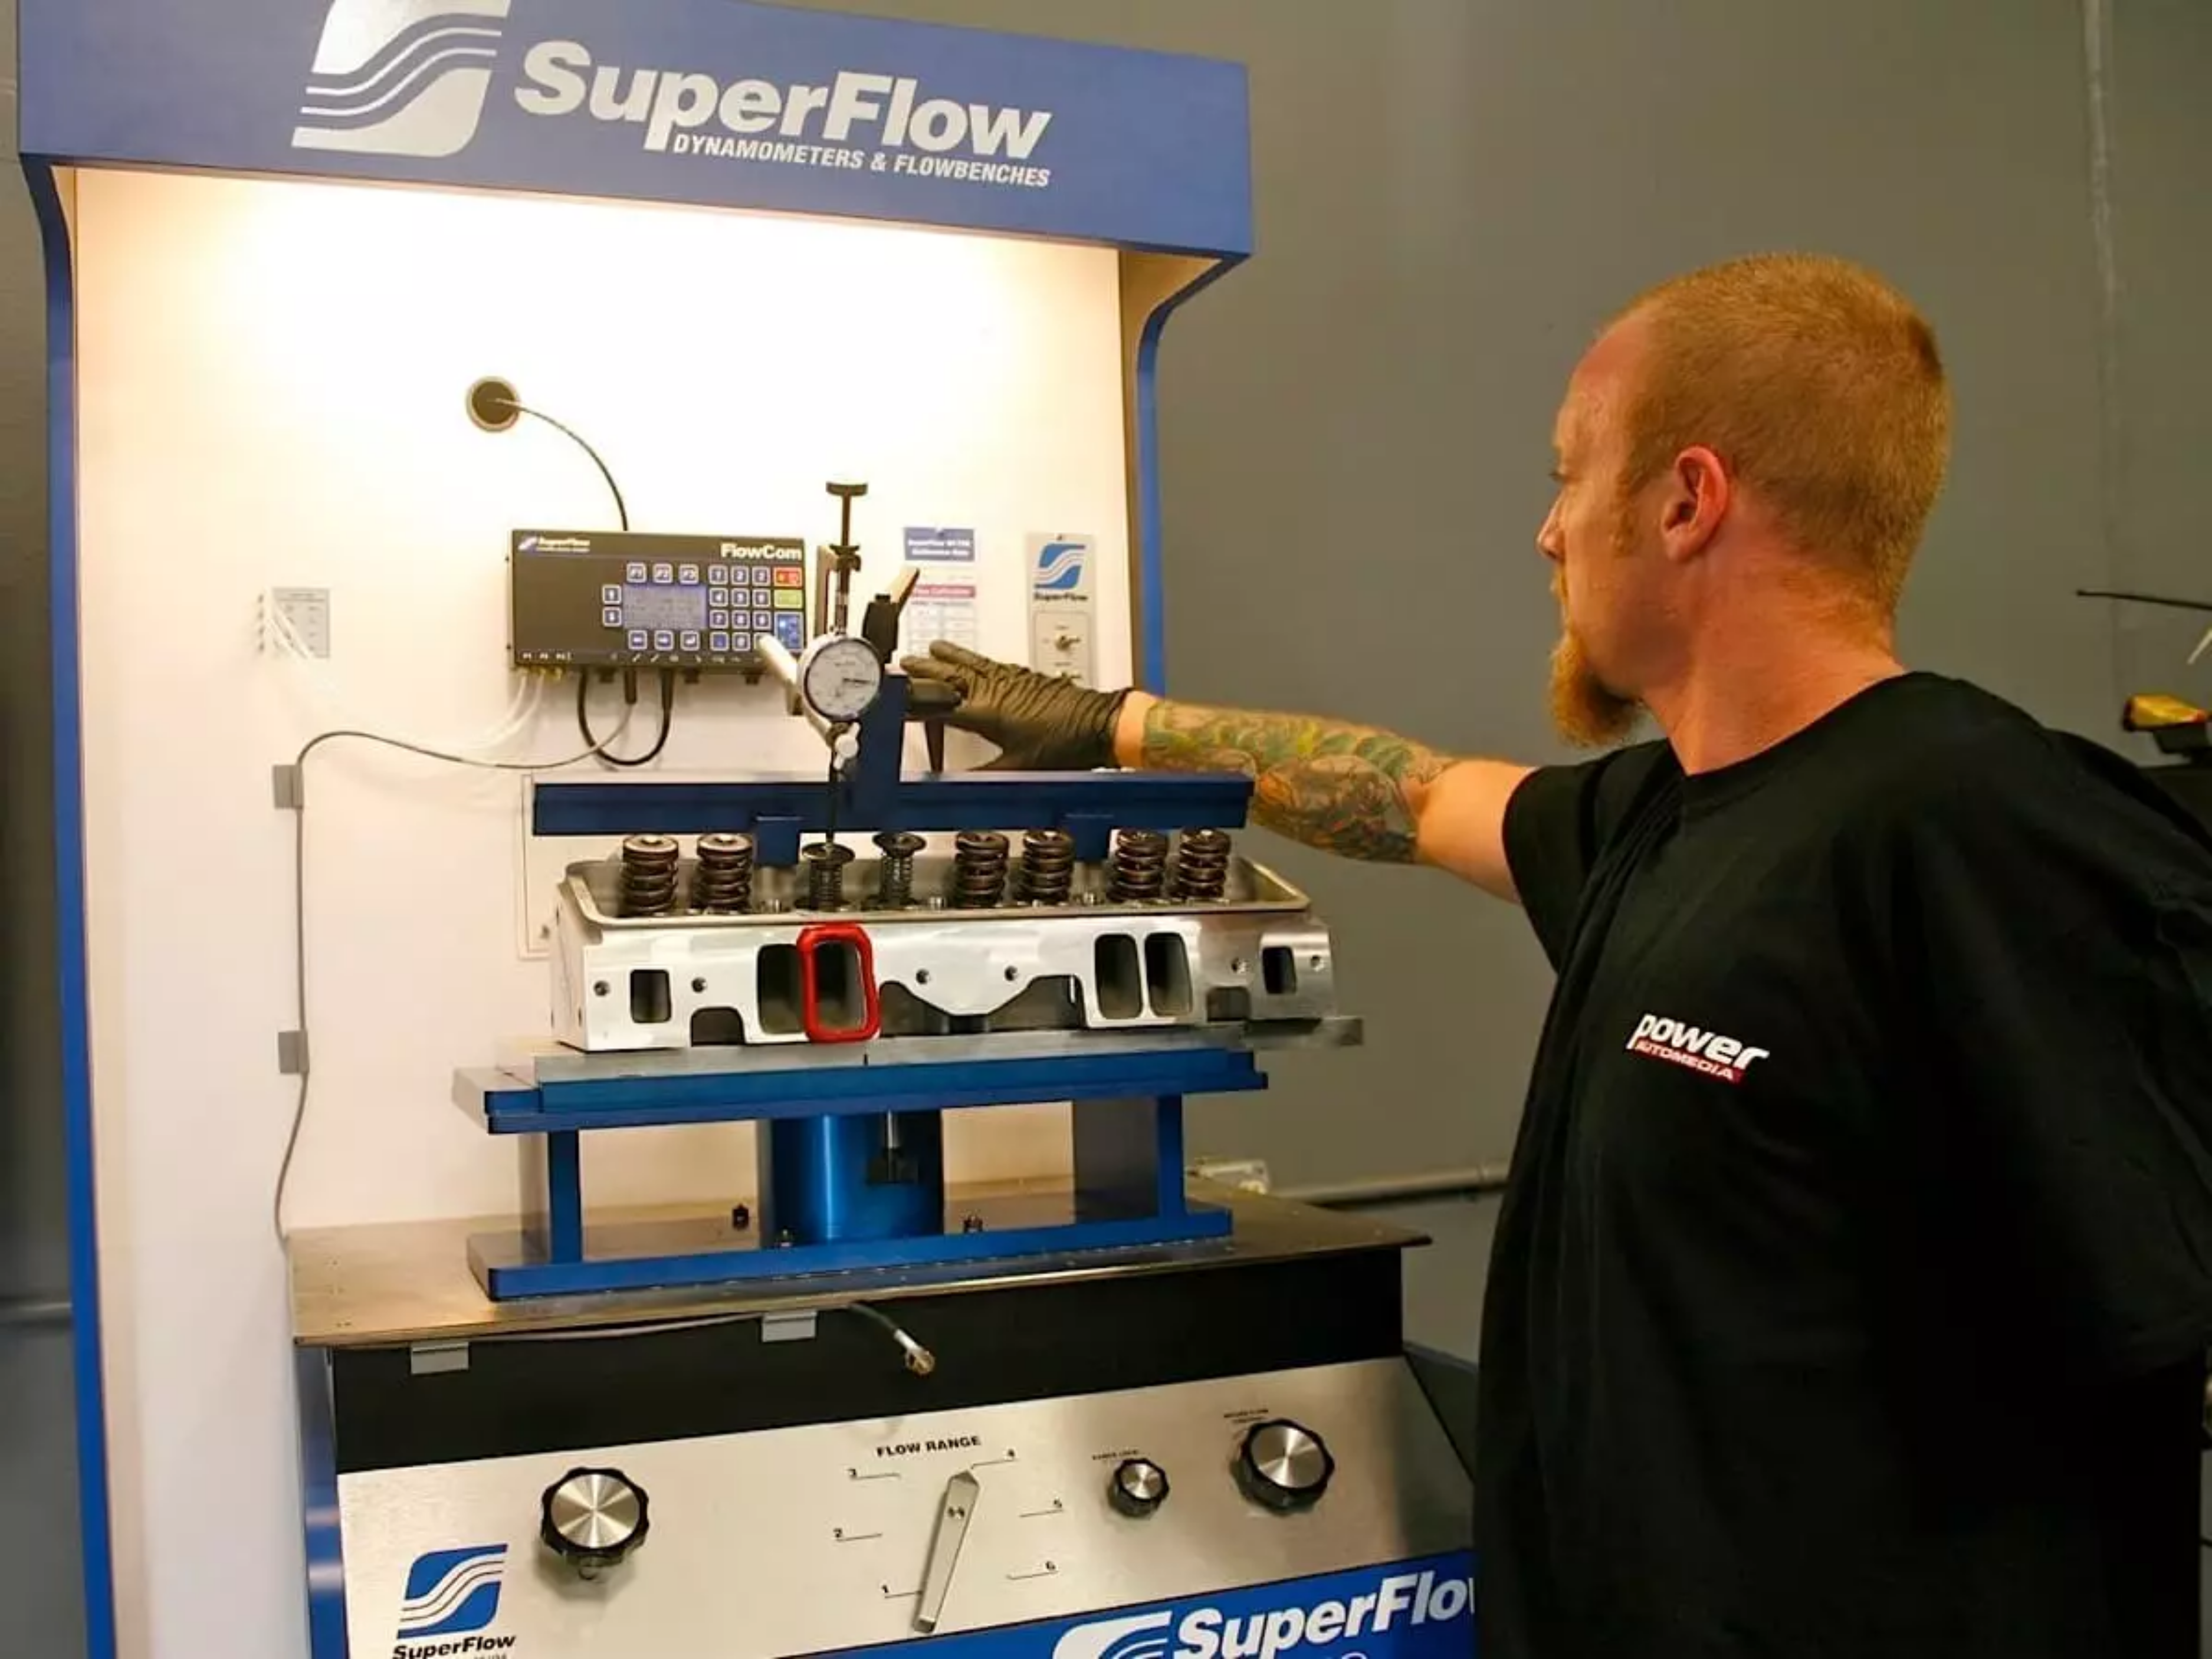
\includegraphics[width=0.5\textwidth]{./flujometrias/banco_flujometrias.png}
%   \caption{Banco de flujometrías Super-Flow SF-750}\label{fig:superflow}
% \end{figure}
%
% Durante el ensayo se mide el caudal de aire atmosférico para diferentes grados
% de apertura de la válvula y así se obtienen datos de (alzada, flujo) con los
% cuales comparar entre diferentes geometrías del puertos de admisión o escape.
% %
% En la Figura~\ref{fig:flow-1} se muestra el resultado del ensayo de un
% flujómetro en el que se compara la capacidad de flujo de dos tapas de cilindro
% diferentes de un BMW S14
% \footnote{\url{http://e30sport.net/tech_articles/engine-tech/flow-1/chart-1.htm}}.
%
% \begin{figure} \centering
% \includegraphics[width=0.8\textwidth]{./flujometrias/flow-1.png}
%   \caption{Comparación entre flujometrías de dos tapas de cilindro de un BMW S14}\label{fig:flow-1}
% \end{figure}
%
% Otra forma de aproximar un coeficiente de descarga es por medio de flujometrías
% computacionales, el uso de CFD permite modelar el puerto en condiciones
% operativas, incluyendo la interacción con elementos como por ejemplo el pistón,
% o en el caso del MRCVC, estator y conjunto rotante.
% %
% Además, se puede modelar las propiedades del fluido de trabajo para una
% viscosidad, presión y temperatura representativas de las condiciones operativas
% del motor que se está modelando.
% %
% En este trabajo se optó por esta metodología, a partir de las flujometrías se
% obtuvo un valor de caudal másico el cual es utilizado para calcular un
% coeficiente de descarga.
%
% A partir de $\dot{m}$, el valor de $C_{D}$  se calcula con de las ecuaciones de
% flujo compresible a través de una restricción, habiendo dos casos distintivos:
% flujo bloqueado y no bloqueado.
%
% Para el caso en que el flujo no esté bloqueado la ecuación de $\dot{m}$ es
% la~(\ref{eq:m_no_bloqueado}) y en caso de que se cumpla la
% desigualdad~(\ref{eq:cond_bloqueo}) el flujo está bloqueado y se utiliza la
% ecuación~(\ref{eq:m_bloqueado}):
% %
%
% \begin{equation}\label{eq:m_no_bloqueado}
%   \dot{m} = \frac{C_D A_R p_0}{\sqrt{R T_0}} {\left(\frac{p_T}{p_0} \right)}^{1/\gamma} {\left( \frac{2\gamma}{\gamma-1} \left[1- {(\frac{p_T}{p_0})}^{{\gamma-1}/\gamma} \right] \right)}^{1/2}
% \end{equation}
%
% \begin{equation}\label{eq:cond_bloqueo}
%   \frac{p_T}{p_0} \le {[\frac{2}{\gamma+1}]}^{\gamma/(\gamma - 1)}
% \end{equation}
%
% \begin{equation}\label{eq:m_bloqueado}
%   \dot{m}=  \frac {C_D A_R p_0} {{(R T_0)}^{1/2}} \gamma^{1/2} {\left( \frac{2\gamma}{\gamma+1} \right)}^{(\gamma+1)/(2(\gamma-1))}
% \end{equation}
%
% donde
% \begin{itemize}
%     \item $p_0$, es la presión de estancamiento antes de la restricción.
%     \item $T_0$, es la temperatura de estancamiento antes de la restricción.
%     \item $p_T$, es la presión estática justo después de la restricción.
%     \item $A_R$, es el área de pasaje de flujo o de referencia.
%     \item $\dot{m}$, es el caudal másico.
%   \item $\gamma$, es el cociente de capacidades térmicas del gas.
% \end{itemize}
%
% \nomenclature[PO]{\(p_0\)}{Presión de estancamiento antes de la restricción}
% \nomenclature[PO]{\(T_0\)}{Temperatura de estancamiento antes de la restricción}
% \nomenclature[PO]{\(p_T\)}{Presión estática justo después de la restricción}
% % \nomenclature[G]{\(A_R\)}{Área de pasaje de flujo o de referencia}
%
% El flujo está bloqueado si la velocidad en la garganta de la restricción alcanza
% la velocidad sónica, dada esta condición $\dot{m}$ alcanza un límite y reducir
% la presión aguas abajo de la restricción no produce un aumento del caudal.
% %
% % La condición de flujo bloqueado se puede expresar en términos de la relación de
% % presiones aguas arriba $p_{0}$ y aguas abajo de la restricción $p_{T}$.
% %
% Las presiones y temperaturas involucradas en el cálculo de $\dot{m}$ se pueden
% medir u obtener de una simulación computacional del ciclo del motor.
% %
% \nomenclature[PO]{\(p,P\)}{Presión}
%
% Un parámetro importante en las ecuaciones utilizadas para el cálculo del
% coeficiente de descarga $C_{D}$ es el área de referencia $A_{R}$ que define el
% área utilizada para calcular el caudal másico que circula por el puerto.
% %
% % En un motor con válvulas se suele tomar el área de cortina como el producto de
% % la circunferencia de la válvula con la alzada, es decir:
%
% La elección del área de referencia utilizada para el cálculo es arbitraria, sin
% embargo en un motor con válvulas se suele utilizar el área de cortina (ver
% Figura~\ref{fig:area_cortina}) la cual es el producto de la circunferencia y la
% alzada de válvula.
%
% \begin{equation} \label{eq:area_cortina}
%   A_R = A_C = \pi D_v l_v
% \end{equation}
%
% % \nomenclature[G]{\(A_R\)}{Área de pasaje de flujo o de referencia}
% \nomenclature[G]{\(A_C\)}{Área de cortina}
% \nomenclature[G]{\(D_v\)}{Diámetro de válvula}
% % \nomenclature[G]{\(l_v\)}{Alzada de válvula}
%
% \begin{figure} \centering
% \includegraphics[width=0.5\textwidth]{valve_curtain.pdf}
%   \caption{Área de cortina}\label{fig:area_cortina}
% \end{figure}
%
% El área de referencia utilizada en ICESym es el área frontal del puerto expuesta
% a la cámara que se esté analizando, calculada como:
%
% \begin{equation}\label{eq:ar_mrcvc}
%   A_{R,i} = h_{p} \cdot l_{v,i}
% \end{equation}
%
% El área de cortina se ilustra en la Figura~\ref{fig:area_cortina} y el área
% utilizada en ICESym para el MRCVC en la Figura~\ref{fig:area_referencia}.
% %
% En esta última figura se observan dos zonas coloreadas, que hacen referencia al
% área de dos cámaras durante el solape que ocurre por la geometría del motor.
%
% \begin{figure}
%   \centering
%   \includegraphics[width=.6\textwidth]{area_referencia.png}
%   \caption{Área de referencia MRCVC}\label{fig:area_referencia}
% \end{figure}
%
% Los valores de densidad, velocidad, presión y temperatura se obtienen de los
% datos de salida de ICESym para un puerto, ángulo y velocidad dada.
% %
% Para la temperatura se utiliza la temperatura de la cámara, $T_0 = T_C$, la
% presión antes y después del puerto se selecciona de acuerdo al sentido de flujo,
% en caso de ser hacia la cámara de combustión la presión en el puerto se utiliza
% como inicial $P_0$ y la presión en la cámara es la aproximación a la presión en
% la restricción $P_T$.
% \nomenclature[PO]{\(T\)}{Temperatura}
% \nomenclature[SU]{\(0\)}{Valor inicial}
%
% El valor de $\gamma$ se obtiene de las propiedades de la mezcla con las rutinas
% computacionales descritas en el apartado~\ref{subsec:prop_mezcla}.


\subsection{Esquemas de Discretización}

Se utilizan para resolver ecuaciones de variables continuas con funciones
discretas en tiempo y espacio.
%
Se deben seleccionar esquemas para resolver:

\begin{itemize}
  \item Primera derivada temporal
  \item Interpolación
  \item Gradiente
  \item Divergencia
  \item Gradientes normales a superficies
  \item Laplacianos
\end{itemize}


\paragraph{Derivadas temporales, $\delta / \delta t$}
%
Estas derivadas se discretizan con el método de Euler\parencite{burden}, que
aproxima la integración de un paso $n$ a $n+1$ con $y_{n+1}-y_{n}\simeq hf_{n}$
donde $h = t_{n+1}-t_{n}$ es el paso temporal y $f_{n}=f(t_{n},y_{n})$.
%
Para el esquema de Euler hacia atrás la aproximación es
$y_{n+1}-y_{n}\simeq h f_{n+1}$.
%
A este esquema se le agrega un coeficiente $\gamma\in[0,1]$ de modo que:

\begin{equation}
  y_{n+1}-y_{n} \simeq \gamma h f_{n+q} + (1-\gamma)h f_{n}
\end{equation}

Con $\gamma=1/2$ el esquema es equivalente a Crank-Nicolson estándar.
%
Se puede convertir al esquema de Euler hacia adelante con $\gamma=0$.

\paragraph{Gradientes}
%
Se discretiza utilizando integración Gaussiana con interpolación lineal entre
valores de celdas.
%
El método define al gradiente medio en un elemento de volumen finito con
centroide \textbf{C} y volumen $V_{c}$ en términos de los flujos a través de sus
caras, como lo indica la ecuación~(\ref{eq:green_gauss_gradient}).
%
Para esto se requiere conocer los valores de la variable $\phi_{f}$ en las caras
vecinas e información del área de la celda y su normal $(\vec{S}_{f})$.

\begin{equation}
  \label{eq:green_gauss_gradient}
  \nabla \phi_{P} = \frac{1}{V_{c}}\sum_{f} \vec{S}_{f}\phi_{f}
\end{equation}

El método de volúmenes finitos utiliza valores en las caras de las celdas, por
lo que se debe aproximar el valor de la variable en una cara dada para obtener
el valor del gradiente en dicha celda.
%
Los valores de $\phi_{f}$ se obtienen de una interpolación lineal entre valores
conocidos de celdas adyacentes.
%
Un método de interpolación entre celdas puede ser:

\begin{align}
  \label{eq:interpolacion_lineal_caras}
  \alpha &= \frac{|{\vec{r}_{N}-\vec{r}_{f}}|} {|{\vec{r}_{N}-\vec{r}_{P}}|}\\
  \phi_{f} &= \alpha\phi_{P}+(1-\alpha)\phi_{N}
\end{align}

Donde $\alpha$ es un factor de ponderación geométrico entre las celdas
\textbf{P} y \textbf{N} y $\vec{r}$ es el vector de posición del centroide de
las celdas.

La interpolación se puede limitar para que los valores obtenidos se encuentren
entre el mínimo y máximo de las celdas vecinas, este método se denomina
``limitado''.


%Gradiente normal a la superficie
\paragraph{Gradiente normal a una superficie}
%
Este gradiente es evaluado en la cara de la celda.
%
Es la componente (normal a la cara) del gradiente entre los valores de los
centroides de 2 celdas conectadas por la cara evaluada.
%
En general las mallas utilizadas para modelar geometrías reales no son
ortogonales.
%
Esto implica que un vector $\vec{S_{f}}$ normal a una superficie no
necesariamente sea colineal con el vector que une el centroide de dos celdas
contiguas.
%
El gradiente en la cara en la dirección que une los centroides (C y F) de las
celdas $\vec{e}$ es

\begin{equation}
  \label{eq:gradiente_normal}
  (\nabla \phi \cdot \vec{e_{f}}) = \frac{\nabla\phi}{\delta n} = \frac{\phi_{F} - \phi_{C}}{||\vec{r_{C}}-\vec{r_{F}}||} = \frac{\phi_{F} - \phi_{C}}{d_{CF}}
\end{equation}

Donde el subíndice $f$ indica que se evalúa en la cara de una celda.
%
El vector de superficie $\vec{S_{f}}$ se puede escribir en términos de sus
componentes normal y tangente a la cara $f$ en la que es evaluado:

\begin{equation}
  \vec{S_{f}}= \vec{E_{f}} + \vec{T_{f}}
\end{equation}

De esta forma, el gradiente del flujo de una variable $\phi$ en mallas no
ortogonales se puede expresar en términos de las componentes normal y tangente a
la cara de la celda~\parencite{moukalled}.
%
El término \textbf{E} indica el flujo de $\phi$ normal a la cara y \textbf{T} el
flujo tangente.

\begin{align}
  \label{eq:gradiente}
  %
  {(\nabla \phi)}_{f}\cdot \vec{S_{f}} &= {(\nabla \phi)}_{f}\cdot E_{f} + {(\nabla \phi)}_{f}\cdot \vec{T_{f}} \\
  %
  &= \vec{E_{f}}\frac{\phi_{F}-\phi_{C}}{d_{FC}}+ {(\nabla \phi)}_{f}\cdot \vec{T_{f}}
\end{align}

%
Algunos esquemas de discretización de este tipo de gradientes son:
\begin{itemize}
  \item No corregido
  \item Ortogonal
  \item Corregido y limitado
\end{itemize}

La corrección ortogonal rota el vector $S_{f}$ hasta que sea normal a la superficie.
%
La corrección limitada aplica la corrección ortogonal, sumando
$\cos^{-1}{\theta}$, donde $\theta$ es el ángulo entre la normal a la cara y el
vector $S_{f}$.

% Divergencia
\paragraph{Divergencia}
%
Se utiliza un esquema de integración Gaussiana con interpolación lineal para
la discretización de la divergencia.

Dependiendo de los tipos de variable, se utilizan diferentes esquemas de
interpolación disponibles, los cuales son:
%
\begin{itemize}
        \item centrada
        \item hacia adelante
        \item hacia atrás
        \item limitada
\end{itemize}

\paragraph{Laplacianos}
%
Los términos Laplacianos se discretizan utilizando integración Gaussiana con
interpolación lineal.



\subsection{Pre-procesado}
%
El preprocesado consiste en definir geometría y condiciones iniciales de la
simulación a partir de los datos obtenidos de las simulaciones con el
optimizador e ICESym.
%
Con los resultados del simulador se grafica la diferencia de presión entre el
puerto de admisión o escape y la cámara correspondiente en función de la apertura
del puerto, para un rango de velocidades de 1000 a 9000 RPM, con el fin de
identificar las zonas en las condiciones operativas en las que evaluar el puerto.
%
En la Figura~\ref{fig:puntos_interes} se muestra una gráfica de $\Delta P$ y
alzada para los puertos de admisión y escape de 1000 a 4000 RPM de un motor
resultante de una de las simulaciones.

Como es de esperarse se tienen mayores diferenciales de presión a menores
aperturas del puerto porque se está próximo a los eventos de apertura o cierre
del mismo.
%
A diferencia del puerto de admisión, en el puerto de escape se ve una banda
bastante definida de operación que se hace más ``llena'' a medida que aumenta la
apertura del puerto.
%
Durante la apertura del puerto se ven las mayores diferencias de presión en las
que hay dos bandas bien definidas.
%
Se toman algunos puntos arriba en la zona con mayor $\Delta P$ y una cantidad
menor para velocidades con $\Delta P \simeq 0$.
%
A medida que el puerto se abre la diferencia de presión con el gas en la cámara
disminuye y esta banda se afina.

\begin{figure}
    \centering
    \includegraphics[width=\textwidth]{gnuplot/puntos_interes.pdf}
    \caption{Presión en función de la apertura el puerto,
$\Delta P = f(l_{v})$}\label{fig:puntos_interes}
\end{figure}

El valor de alzada está directamente relacionado con la posición angular del
cigüeñal, por lo que una vez seleccionados los puntos de interés se puede
extraer la geometría deseada de un modelo de CAD paramétrico del motor.
%
En este modelo se representó la mitad de la geometría que contiene los puertos
de admisión y escape, y se obtuvo realizando operaciones geométricas con los
volúmenes que representan diferentes componentes del motor como son el estator,
rotor, paletas, etc.
%
% En la Figura~\ref{fig:admision_50} se muestra parte del proceso para obtener el
% puerto de admisión a $\theta=50^{\circ}$, en donde se suma el volumen del mismo
% en gris y las Figuras que se restan que corresponden al rotor, las paletas y un
% paralelogramo para quitar una región que no se simuló.

\begin{figure}
    \centering
    \includegraphics[width=0.7\textwidth]{./CAD/freecad_pasos.png}
    \caption{Puerto de admisión para $\theta=50^{\circ}$ modelado con
FreeCAD}\label{fig:admision_50}
\end{figure}

Esta geometría fue generada por el programa FreeCAD~\parencite{freecad},
exportada a un archivo
``.BREP''\footnote{\href{https://dev.opencascade.org/doc/overview/html/specification\_\_brep\_format.html}{Formato
BREP, opencascade.org}} para luego ser importada en Salome\parencite{salome},
que se utiliza para generar una malla cerrada, hermética, que puede ser
procesada por los complementos de OpenFOAM utilizados para generar la malla de
la simulación.
%
Es importante que se satisfaga la hermeticidad de la malla, lo cual significa
que los nodos en la frontera entre superficies coincidan, como se puede observar
en la Figura~\ref{fig:salome_malla_hermetica}, en la que se ven dos superficies
``walls'' y ``outlet'' y los nodos compartidos entre ambas superficies.
%

\begin{figure}[ht]
    \centering
    \includegraphics[width=0.4\textwidth]{./flujometrias/salome_malla_hermetica.png}
    \caption{Malla hermética}\label{fig:salome_malla_hermetica}
\end{figure}

El proceso en Salome consta de importar la geometría generada por FreeCAD y
separar la misma en superficies utilizadas para definir condiciones de contorno
en OpenFOAM.
%
Las superficies diferenciadas son: puerto, cámara/s y pared, ver
Figura~\ref{fig:openfoam_parches}.

\begin{figure}[ht]
    \centering
    \includegraphics[width=0.5\textwidth]{./flujometrias/openfoam_parches.png}
    \caption{Nombres de Parches}\label{fig:openfoam_parches}
\end{figure}

Luego de separadas estas superficies se procede a generar la malla en formato
ASCII STL con el complemento de mallado de Salome.
%
Se utilizó el generador de mallas NETGEN 1D-2D para crear la superficie, en
general se configuró el software de modo de tener un stl de buena calidad con
elementos de menor tamaño en zonas de mayor curvatura.
%
En la Figura~\ref{fig:salome_fina_gruesa} se ve la diferencia en cantidad de
nodos de dos mallas, una malla fina a la izquierda y una malla gruesa a la
derecha.
%
En la Tabla~\ref{tab:salome_fina_gruesa} se muestra la diferencia entre algunos
parámetros básicos de configuración para las dos mallas.
%
% Esto sin requerir de una gran cantidad de elementos para no ralentizar el
% procesado con SnappyHexMesh.

\begin{figure}[t!]
    \centering
    \begin{subfigure}[t]{0.5\textwidth}
        \centering
        \includegraphics{/flujometrias/salome3_fina.png}
        \caption{Malla fina sin optimizar}
    \end{subfigure}%
    \begin{subfigure}[t]{0.5\textwidth}
        \centering
        \includegraphics{/flujometrias/salome3_gruesa.png}
        \caption{Malla gruesa optimizada}
    \end{subfigure}
    \caption{Diferentes mallas para flujometrías}\label{fig:salome_fina_gruesa}
\end{figure}

\begin{table}
    \centering
    \begin{tabular}{lccc} \toprule
        Parámetro                & Malla Fina    & Malla Gruesa     & Unidades\\ \midrule
        Tamaño máximo            & 0,001         & 0,03             & m \\
        Tamaño mínimo            & 1E-7          & 2,4E-5           & m \\
        Limitado por curvatura   & Sí            & Sí               & - \\
        Optimizar                & No            & Sí               & - \\
        Cantidad de nodos        & 99311         & 49112            & - \\
        Cantidad de elementos    & 204695        & 103163           & - \\ \bottomrule
    \end{tabular}
    \caption{Configuración de mallas mostradas en la Figura~\ref{fig:salome_fina_gruesa}}
    \label{tab:salome_fina_gruesa}
\end{table}
